% (c) 2014 Claudio.carboncinii - claudio.carboncini@gmail.com
% (c) 2014 Dimitrios Vrettos - d.vrettos@gmail.com
\chapter{Numeri reali}
\section{Dai numeri naturali ai numeri irrazionali}
Nel volume Algebra 1 abbiamo presentato i diversi insiemi numerici. Li 
riprendiamo brevemente per poi approfondire i numeri reali e le loro proprietà.

L'insieme dei \emph{numeri naturali} racchiude i numeri che utilizziamo per 
contare; si indica nel seguente modo:
\[\insN=\{0,1,2,3,4,5,6,7,8,9,10,11,\ldots\}\]

Su questi numeri sono definite le seguenti operazioni:
\begin{itemize*}
 \item \emph{addizione}: $n+m$ è il numero che si ottiene partendo da $n$ e 
  continuando a contare per altre $m$ unità;
 \item \emph{sottrazione}: $n-m$ è il numero, se esiste, che 
  addizionato a $m$ dà come risultato $n$;
 \item \emph{moltiplicazione}: $n \cdot m$ è il numero che si ottiene sommando 
  $n$ volte $m$, o meglio sommando $n$ addendi tutti uguali a $m$
 \item \emph{divisione}: $n:m$ è il numero, se esiste, che 
  moltiplicato per $m$ dà come risultato $n$;
 \item \emph{potenza}: $n^{m}$ è il numero che si ottiene moltiplicando $m$ 
  fattori tutti uguali a $n$ con $m \ge 2$, ponendo $n^{1}=n$ e $n^{0}=1$;
 \item \emph{radice}: $\sqrt[{n}]{m}$ con $n\ge 2$ è il numero, se esiste, 
  che elevato a $n$ dà come risultato $m$.
\end{itemize*}

L'addizione, la moltiplicazione e la potenza sono definite su tutto l'insieme 
dei numeri naturali, cioè dati due numeri naturali qualsiasi, $n$ ed $m$, la 
somma $n+m$ e il loro prodotto $n \cdot m$ e la loro potenza $n^{m}$, 
escluso il caso $0^{0}$, danno come risultato un numero naturale. 
Non sempre invece, la differenza $n-m$, il quoziente $n:m$ o la 
radice $\sqrt[{n}]{m}$ di due numeri naturali danno come risultato un numero 
naturale.

Tuttavia, dal punto di vista pratico-applicativo molto spesso si incontrano 
situazioni nelle quali occorre eseguire sempre operazioni. Iniziamo 
dall'operazione di sottrazione. Sappiamo che in tante situazioni di natura 
economica, ma non solo, deve essere possibile sottrarre un numero da uno più 
piccolo. Deve essere possibile, per esempio, comprare un'auto che costa 12.000 
euro anche quando in banca possediamo solo 10.000 euro. Deve quindi essere 
possibile eseguire una sottrazione del tipo $10.000-12.000$. Il risultato di 
questa operazione non va poi confuso con il risultato di $12.000-10.000$. Nel 
secondo caso, infatti, significa che sul nostro conto corrente abbiamo 12.000 
euro e dobbiamo spenderne 10.000, ci rimangono quindi 2.000 euro. Nel primo caso 
invece, possediamo 10.000 euro e dobbiamo pagare
12.000 euro ci rimane un debito di 2.000 euro. Per distinguere i due tipi di 
numeri i matematici mettono davanti al numero il segno $+$ o il segno $-$. Si 
genera così l'insieme dei \emph{numeri interi}.
\[\insZ=\{\ldots,-3,-2,-1,0,+1,+2,+3,\ldots\}\]

Su questi numeri l'operazione di sottrazione è ovunque definita, in altre parole 
il risultato di qualunque sottrazione tra due numeri interi è un numero intero.

Non è invece possibile eseguire sempre le divisioni. Oltre hai casi $n:0$ e 
$0:0$ che non sono definiti, solo in casi particolari è possibile dividere 
due numeri interi e ottenere come risultato un numero intero. Ad esempio $5:4$ 
non ha un risultato all'interno dell'insieme dei numeri interi. 
Esistono però tante situazioni reali in cui una divisione di questo tipo deve 
poter essere eseguita. Per esempio è possibile dividere in parti uguali 5 uova 
in 4 persone, basta fare una frittata in una padella tonda e dividere la 
frittata in quattro parti uguali, a ciascuna toccano $\frac{5}{4}$ di uovo. Deve
essere possibile dividere in parti uguali 5 euro tra 4 persone. 
In tutto a ciascuno toccano 1 euro e 25 centesimi di euro: $1,25$.

Per rappresentare il risultato di queste due operazioni di divisioni abbiamo 
usato nel primo caso la notazione frazionaria $\frac{5}{4}$ e nel secondo caso 
la notazione decimale $1,25$. Le due scritture sono perfettamente equivalenti.

Per risolvere tutti i problemi di divisione i matematici hanno costruito 
l'insieme dei \emph{numeri razionali} che indichiamo nel seguente modo:
\[
\insQ=\left\{\frac{n}{m} \mid n\in \insZ,m\in \insN,m\neq
0\right\}=\left\{0,+1,-1,\frac{1}{2},-\frac{1}{2},+\frac{2}{3,}-\frac{1}{5},
-\frac{11}{17},\frac{129}{1725}...\right\}
\]

Con questi numeri è possibile sempre eseguire l'addizione, la sottrazione, la 
moltiplicazione, la divisione (ad eccezione della divisione per 0), la potenza. 
Non sempre, invece, è possibile eseguire l'estrazione di radice. Per esempio, 
hai già conosciuto il numero $\sqrt{2}$, cioè il numero che elevato al quadrato 
dà 2; esso non è un numero razionale, cioè non può essere scritto né sotto forma 
di frazione né sotto forma di numero decimale finito o periodico. I numeri di 
questo tipo si dicono \emph{numeri irrazionali}.

Abbiamo già affrontato questo problema nel volume di Algebra 1; per comodità del 
lettore riportiamo il ragionamento.

Fissiamo sulla retta orientata~$r$ l'unità di misura e disegniamo il quadrato di 
lato~1. Ci proponiamo di calcolare
la misura della sua diagonale~$OB$.

\begin{center}
 % (c) 2013 Claudio Carboncini - claudio.carboncini@gmail.com
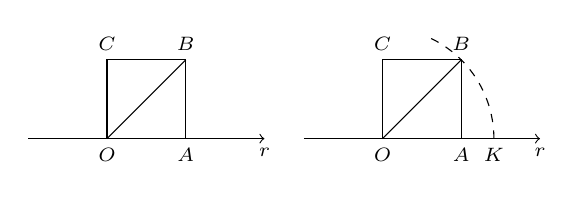
\begin{tikzpicture}[x=10mm, y=10mm, font=\scriptsize]
  \draw [->] (0,0) -- (3,0) node [below] () {$r$};
  \draw (1,0) rectangle (2,1);
  \draw (1,0) -- (2,1);

  \coordinate[label=below:$O$] (O) at (1,0);
  \coordinate[label=below:$A$] (A) at (2,0);
  \coordinate[label=above:$C$] (C) at (1,1);
  \coordinate[label=above:$B$] (B) at (2,1);

  \begin{scope}[xshift=35mm]
    \draw [->] (0,0) -- (3,0) node [below] () {$r$};
    \draw (1,0) rectangle (2,1);
    \draw (1,0) -- (2,1);

    \coordinate[label=below:$O$] (O) at (1,0);
    \coordinate[label=below:$A$] (A) at (2,0);
    \coordinate[label=above:$C$] (C) at (1,1);
    \coordinate[label=above:$B$] (B) at (2,1);
    \coordinate[label=below:$K$] (K) at (2.414,0);

    \draw[dashed] (2.414,0) arc [start angle=0, end angle=65,radius=1.414cm,];

  \end{scope}
\end{tikzpicture}

\end{center}

Il triangolo~$OAB$ è retto in~$A$, quindi per il teorema di
Pitagora~$\overline{OB}^{2}=\overline{OA}^{2}+\overline{AB}^{2}$.
Sostituiamo le misure:~$\overline{OB}^{2}=1^2+1^2=2$. Per 
ottenere~$\overline{OB}$
dobbiamo estrarre la radice quadrata e quindi~$\overline{OB}=\sqrt{2}$.

Sappiamo che ``estrarre la radice quadrata'' di un numero, detto radicando, 
significa trovare quel numero che elevato al quadrato dà come risultato
il radicando. 
Questo numero deve esistere, nel senso
che esiste un punto sulla retta~$r$ che lo rappresenta, per costruirlo 
graficamente si può tracciare l'arco di
circonferenza di centro~$O$ e raggio~$OB$ determinando su $r$ il punto~$K$ 
estremo del segmento con~$OK = OB$.

Dalla posizione del punto~$K$ possiamo dire che~$1<\sqrt{2}<2$. Il
valore cercato evidentemente non è un numero intero. Può essere un
numero decimale finito? Compiliamo una tabella che contenga nella prima
riga i numeri con una sola cifra decimale compresi tra~1 e~2 e nella
seconda riga i rispettivi quadrati:

\begin{center}
\begin{tabular}{ccccccc}
\toprule
$x$ & 1,1 & 1,2 & 1,3 & 1,4 & 1,5 & 1,6\\
$x^{2}$ & 1,21 & 1,44 & 1,69 & 1,96 & 2,25 & 2,89\\
\bottomrule
\end{tabular}
\end{center}

Osserviamo che il numero~2 è compreso tra~$1,4^{2}$ e~$1,5^{2}$,
di conseguenza~$1,4<\sqrt{2}<1,5$, ma ancora
non possiamo precisare il suo valore, anche se abbiamo ristretto
l'intervallo in cui si trova il punto~$K$. Diciamo che~1,4 è un valore 
approssimato per
difetto di~$\sqrt{2}$ mentre~1,5
è un valore approssimato per eccesso; scrivendo~$\sqrt{2}=1,4$
oppure~$\sqrt{2}=1,5$ commettiamo un errore minore di~1/10.

Per migliorare l'approssimazione e tentare di ottenere~$\sqrt{2}$
come numero razionale costruiamo la tabella dei numeri
decimali con due cifre compresi tra~1,4 e~1,5:

\begin{center}
\begin{tabular}{ccccc}
\toprule
$x$ &1,41 &1,42 &1,43 &1,44\\
$x^{2}$ & 1,9881 & 2,0164 & 2,0049 & 2,0776\\
\bottomrule
\end{tabular}
\end{center}

Ora possiamo dire che~1,41 è un valore approssimato per difetto di~$\sqrt{2}$ 
mentre~1,42 è un valore approssimato
per eccesso, con un errore dell'ordine di~1/100. Abbiamo quindi migliorato
l'approssimazione e di conseguenza abbiamo ristretto l'intervallo in cui cade il 
punto~$K$, ma ancora non
abbiamo trovato un numero razionale che sia uguale a~$\sqrt{2}$.

Continuando con lo stesso procedimento costruiamo due classi di numeri razionali 
che approssimano una per difetto e
una per eccesso il numero cercato, restringendo ogni volta l'ampiezza 
dell'intervallo in cui cade il punto~$K$.
Il procedimento può continuare all'infinito e le cifre decimali che troviamo non si 
ripetono periodicamente.

\begin{center}
 \begin{tabular}{rcll}
\toprule
Valore per difetto & Numero &Valore per eccesso & Ordine dell'errore\\
\midrule
1 & $\sqrt{2}$  & 2  & $10^{0}$\\
1,4 & $\sqrt{2}$ & 1,5  & $10^{-1}$\\
1,41 & $\sqrt{2}$ & 1,42 & $10^{-2}$\\
1,414 & $\sqrt{2}$ &1,415 & $10^{-3}$\\
1,4142 & $\sqrt{2}$ & 1,4143 & $10^{-4}$\\
\ldots & $\sqrt{2}$ & \ldots & \ldots\\
\bottomrule
\end{tabular}
\end{center}

Si può dimostrare che~$\sqrt{2}$ non è un numero razionale con una elegante 
dimostrazione per assurdo. 

% \begin{itemize*}
%  \item 
% Supponiamo che la radice di due sia un numero razionale scritto sotto forma di 
% frazione~$\sqrt{2}= \frac{a}{b}$, Certamente possiamo ridurre la frazione ai 
% minimi termini.
%  \item 
% Se si elevano al quadrato entrambi i membri dell'equazione precedente, si 
% ottiene:~$2=\frac{a^{2}}{b^{2}}$.
%  \item
% La precedente uguaglianza può anche essere scritta come $2 \cdot b^2 = a^2$, 
% da cui si deduce che $a^2$ è un numero pari. Ma se $a^2$ è pari lo deve essere 
% anche $a$.
% quindi $a$ può essere visto come il doppio di un numero:~$a=2 \cdot k$.
%  \item 
% L'uguaglianza precedente può essere vista come:~$2 \cdot b^2 = (2 \cdot k)^2$.
% Elevando al quadrato il monomio di destra si 
% ottiene:~$2 \cdot b^2 = 4 \cdot k^2$.
%  \item 
% Dividendo per 2 entrambi i membri dell'uguaglianza 
% otteniamo:~$b^2 = 2 \cdot k^2$. Da questo discende che anche~$b^2$ è pari e 
% quindi anche $b$, ma se sono entrambi pari allora la frazione di partenza è
% riducibile contraddicendo che la frazione di partenza fosse ridotta ai minimi 
% termini.
% \end{itemize*}

Elevare un numero al quadrato significa elevare al quadrato le
singole potenze dei fattori primi in cui questo si scompone. I fattori
primi di~$a^{2}$ e di~$b^{2}$ sono gli stessi di~$a$ e di~$b$ con
gli esponenti raddoppiati, Se~$a$ e~$b$ non hanno fattori in comune, 
anche~$a^{2}$ e~$b^{2}$ non li avranno. Quindi ~$a^{2}$ non può essere il 
doppio di~$b^{2}$.
Perciò~$2\ne\frac{a^{2}}{b^{2}}$ e~$\sqrt{2}\ne\frac{a}{b}$.

Oltre a $\sqrt{2}$ vi sono altri infiniti numeri che non possono essere scritti 
come frazione. Molte radici e alcuni numeri particolari come $\pi$, 
che corrisponde alla misura della circonferenza di diametro $1$.

Questi numeri sono detti \emph{numeri irrazionali} e costituiscono l'insieme 
$\insJ$ dei numeri irrazionali.

L'unione degli insiemi $\insQ$ e $\insJ$ è l'insieme $\insR$ dei numeri reali.

% \vspazio\ovalbox{\risolvii \ref{ese:1.1}, \ref{ese:1.2}}

\section{I numeri reali}
In base a quanto abbiamo detto prima, essendo $\insR=\insQ \cup \insJ$, i numeri 
reali sono tutti quei numeri che si possono scrivere in forma decimale con un 
numero finito o infinito di cifre, non necessariamente periodiche.
Per esempio, la frazione $\dfrac{17}{16}$ è uguale al numero decimale 
finito~1,0625.
La frazione $\dfrac{16}{17}$ è uguale al numero decimale periodico 
$0,\overline{9411764705882352}$.

Il numero $\pi$ è invece un numero decimale a infinite cifre non periodico. 
Riportiamo alcune cifre:
$\pi $ = 3, 141 592 653 589 793 238 462 643 383 279 502 884 197 169 399 375 105 
820 974 944 592 307 816 406 286
% 208 998 628 034 825 342 117 067 982 148 086 513 282 306 647 093 844 609 550 582 
% 231 725 359 408 128 481 117 450 284 102
% 701 938 521 105 559 644 622 948 954 930 381 964 428 810 975 665 933 446 128 475 
% 648 233 786 783 165 271 201 909 145 648
% 566 923 460 348 610 454 326 648 213 393 607 260 
\ldots Nonostante i numeri 
irrazionali siano stati scoperti dallo stesso Pitagora o dai suoi allievi nel 
$IV$~secolo~$\aC$, solo nel $XIX$~secolo Augustin-Louis Cauchy e Richard 
Dedekind sono giunti a una formulazione rigorosa di numeri reali.

In effetti, assumere che i numeri reali sono tutti quelli che si possono 
scrivere in forma decimale finita o infinita,  comporta dei problemi. 
Per esempio, gli algoritmi per addizionare, 
sottrarre e moltiplicare due numeri richiedono di cominciare dalla cifra 
più a destra, cosa che non è possibile per i numeri decimali che non 
finiscono mai. 

È possibile costruire l'insieme dei numeri reali a 
partire dall'insieme dei numeri razionali dividendoli in due insiemi~$A$ e~$B$ 
con particolari caratteristiche:
\begin{enumerate*}
 \item $A \cap B=\emptyset$
 \item $A \cup B=\insQ$
 \item $\forall a \in A, \forall b \in B, a<b$
\end{enumerate*}

Una coppia di insiemi con queste caratteristiche venne chiamato da 
Dedekind~(1831-1916) una \emph{sezione}, o \emph{partizione} di $\insQ$.

Dato che $A$ e $B$ devono avere intersezione nulla:

\begin{itemize*}
 \item se $A$ ha un massimo $B$ non può avere un minimo;
 \item se $A$ non ha un massimo $B$ può avere un minimo;
 \item $A$ può non avere un massimo $B$ può non avere un minimo;
\end{itemize*}

% Nei primi due casi La sezione individua un numero Razionale, nel terzo caso,
% individua un numero irrazionale.

\begin{exrig}
 \begin{esempio}
 Sezioni
 \begin{itemize}
 \item I due insiemi $A$ e $B$ così definiti: 
 $A=\left\{x\in \insQ |\, x<3\right\}$ e
$B=\left\{x\in \insQ |\, x \ge 3\right\}$ 
definiscono una sezione di $\insQ$, 
infatti $A \cap B=\emptyset$ $A \cup B=\insQ$ e ogni elemento di A è minore 
di ogni elemento di B; 
inoltre possiamo osservare che $A$ non ammette massimo,
non essendoci in esso un numero che sia maggiore di tutti gli altri, 
mentre $B$ ammette il minimo che è 3;
 \item siano $A=\left\{x\in \insQ |\, x<-1\right\}$, $B=\left\{x \in \insQ |\, 
x>0\right\}$ la coppia $(A,B)$ non è una sezione di $\insQ$ perché pur essendo 
$A\cap B=\emptyset$ non è $A\cup B=\insQ$
 \item siano $A=\left\{x\in \insQ |\, x \le \frac{2}{7}\right\}$, $B=\left\{x 
\in Q |\, x \ge \frac{2}{7}\right\}$, anche in questo caso la coppia $(A,B)$ non 
è una sezione di $\insQ$ poiché $A\cap B=\left\{\frac{2}{7}\right\}$
 \item costruiamo gli insiemi $A$ e $B$ nel seguente modo: $A$ sia l'unione tra 
l'insieme dei numeri razionali negativi e tutti i razionali il cui quadrato è 
minore di 2, in $B$ mettiamo tutti i razionali il cui quadrato è maggiore di 2. 
$A=\insQ^{-} \cup \left\{x \in \insQ |\, x^{2}<2\right\}$, $B=\left\{x \in \insQ 
|\, x^{2}>2\right\}$. Si ha $A \cap B=\emptyset$ $A\cup B=\insQ$, inoltre ogni 
elemento di $A$ è minore di ogni elemento di $B$, dunque $(A,B)$ è una sezione 
di $\insQ$, ma $A$ non possiede il massimo e $B$ non possiede il minimo, in 
quanto abbiamo già dimostrato che non esiste un numero razionale che ha $2$ come 
quadrato. Questa sezione individua un buco nell'insieme $\insQ$.
 \end{itemize}
 \end{esempio}
\end{exrig}

\begin{definizione}
Si chiama \emph{elemento separatore} di una partizione $(A,B)$ di $\insQ$ il 
massimo di $A$ o il minimo di $B$, nel caso in cui almeno uno di questi elementi 
esista.
\end{definizione}

Nel primo esempio, poiché esiste il minimo di $B$, la partizione $(A,B)$ ammette 
un elemento separatore e identifica il numero razionale $3$.
Nel quarto esempio non esiste un numero razionale che fa da elemento separatore, 
la sezione $(A,B)$ identifica un numero irrazionale.

\begin{definizione}
L'insieme $\insR$ dei numeri reali è l'insieme di tutte le partizioni di 
$\insQ$. Chiamiamo
numero razionale le partizioni che ammettono elemento separatore, chiamiamo 
\emph{numero irrazionale} le sezioni che non ammettono elemento separatore.
\end{definizione}

Ogni numero reale è individuato da due insiemi di numeri razionali che 
contengono, nel primo tutte le approssimazioni per difetto e il secondo
tutte le approssimazioni per eccesso.

% Ritornando all'esempio precedente, il numero $\sqrt{2}$ è individuato dalla 
% sezione costituita dagli insiemi $A=\left\{x\in \insQ |\, x<0\right\}$ oppure 
% $x^{2}<2$ e $B=\left\{x\in \insQ |\, x^{2}>2\right\}$.
% Nell'insieme $A$ ci sono tutti i numeri razionali negativi oltre quelli che 
% approssimano $\sqrt{2}$ per difetto: 
% \[A=\{1;1,4;1,41;1,414;1,4142;1,414213;\ldots\}.\]
% Nell'insieme B ci sono tutti i numeri razionali che approssimano $\sqrt{2}$ per 
% eccesso:
% \[B=\{2;1,5;1,42;1,415;1,4143;1,41422;1,414214;\ldots\}.\]

Questa costruzione dell'insieme dei numeri reali $\insR$ a partire 
dall'insieme dei numeri razionali $\insQ$ è puramente astratta e formale, 
non serve al calcolo, ma
permette di collegare i nuovi numeri all'insieme dei numeri naturali $\insN$. 

Nell'insieme delle partizioni di $\insQ$ è possibile definire in modo rigoroso 
l'ordinamento e le operazioni, nella pratica si usano sempre delle 
approssimazioni, magari molto elevate.

\begin{definizione}
Un insieme $X$ si dice \emph{continuo} se ogni partizione $(X', X'')$ di $X$ 
ammette uno e un solo elemento separatore, cioè se esiste un elemento $x$ 
appartenente a $X$ tale che per ogni $x'$ di $X'$ e per ogni $x''$ di $X''$ si 
ha $x'{\leq}x{\leq}x''$.
\end{definizione}

\begin{teorema}[di Dedekind]
Ogni partizione dell'insieme $\insR$ di numeri reali ammette uno e uno solo 
elemento separatore.
\end{teorema}

Da questo teorema segue che il numero reale è definito come l'elemento 
separatore di una sezione $(A,B)$ di numeri reali.

\begin{postulato}[di continuità della retta]
Esiste una corrispondenza biunivoca tra l'insieme dei punti della retta 
geometrica e l'insieme $\insR$ dei numeri reali.
\end{postulato}

Da questo postulato segue la possibilità di definire sulla retta un sistema di 
coordinate: ad ogni punto corrisponde un numero reale (la sua ascissa) e 
viceversa ad ogni numero reale è associato uno e un solo punto sulla retta; 
analogamente si ha nel piano dove il sistema di assi cartesiano permette di 
realizzare una corrispondenza biunivoca tra coppie di numeri reali (ascissa e 
ordinata del punto) e un punto del piano geometrico. Vedremo in seguito che la 
possibilità di associare numeri e punti si estende anche allo spazio geometrico.

% \subsection{Confronto fra numeri reali}
% Per confrontare due numeri reali, osserviamo prima di tutto i segni. Se i segni 
% dei numeri sono
% discordi, il numero negativo è minore del numero positivo. Se i segni dei numeri 
% sono concordi si valuta la parte intera del numero: se sono positivi è più 
% grande quello che ha la parte intera maggiore, viceversa se sono negativi è più 
% grande quello che ha la parte intera minore. A parità di parte intera bisogna 
% confrontare la parte decimale partendo dalle cifre più a sinistra finché non si 
% trova la prima cifra decimale diversa: se i numeri sono positivi è maggiore 
% quello che ha la cifra maggiore; se sono negativi è maggiore quello che ha la 
% cifra minore.
% 
% \begin{exrig}
%  \begin{esempio}
%  Confrontare i seguenti numeri reali
%  \begin{itemize}
%  \item $\sqrt{2}<\sqrt{3}$ per verificarlo ci si può aiutare con la calcolatrice 
% per calcolare le prime cifre decimali dei due numeri $\sqrt{2}=1,4142\ldots$, 
% $\sqrt{3}=1,7320\ldots$ oppure ci si arriva osservando che il numero che elevato 
% al quadrato dà 2 deve essere minore del numero che elevato al quadrato dà 3;
%  \item $\sqrt{99}<10$ per verificarlo è sufficiente osservare che 
% $\sqrt{100}=10$.
%  \end{itemize}
%  \end{esempio}
% \end{exrig}

% \ovalbox{\risolvii \ref{ese:1.3}, \ref{ese:1.4}, \ref{ese:1.5}, \ref{ese:1.6}, 
% \ref{ese:1.7}}\vspazio

\section{Richiami sul valore assoluto}

Si definisce \emph{valore assoluto} di un numero reale $a$, indicato con 
$\valass{a}$, il numero stesso se $a$ è positivo o nullo, il suo opposto se $a$ 
è negativo.

\[
|a|=\left\{\begin{array}{lcc}
 a & \text{, se } & a\ge~0\\
-a & \text{, se } & a<0\end{array}.\right.
\]

Il numero $a$ si dice argomento del valore assoluto.
\begin{multicols}{3}
$\valass{-3}=3$\\$\valass{+5}=5$\\$\valass{0}=0$.
\end{multicols}
\subsection{Proprietà del valore assoluto}
$\valass{x+y}\le \valass{x}+\valass{y}$: il valore assoluto della somma di due 
numeri è minore o uguale della somma dei valori assoluti dei due numeri. Si ha 
l'uguaglianza solo quando i due numeri reali hanno lo stesso segno, oppure 
quando almeno uno dei due numeri è nullo.

$\valass{x-y}\le \valass{x}+\valass{y}$: il valore assoluto della differenza di 
due numeri è minore o uguale della somma dei valori assoluti dei due numeri.

$\valass{x\cdot y}=\valass{x}\cdot \valass{y}$: il valore assoluto del prodotto 
di due numeri
è uguale al prodotto dei valori assoluti dei due numeri.

$\left |{\dfrac{x}{y}}\right|=\dfrac{\valass{x}}{\valass{y}}$: il valore 
assoluto del rapporto di due
numeri è uguale al rapporto dei valori assoluti dei due numeri.

In generale, se l'argomento del valore assoluto è una funzione $f(x)$ si ha:
\[
\valass{f(x)}=\left\{\begin{array}{lcc}
 f(x) & \text{, se } & f(x)\ge~0\\
-f(x) & \text{, se } & f(x)<0\end{array}.\right.
\]
\begin{exrig}
 \begin{esempio}
 Valore assoluto di numeri reali
 \begin{itemize}
 \item $\valass{5+3}=\valass{5}+\valass{3}$ in entrambi i casi si ottiene $8$
 \item $\valass{5+(-3)}=2$ mentre $\valass{5}+\valass{-3}=8$, pertanto 
$\valass{5+(-3)}<\valass{5}+\valass{-3}$.
 \end{itemize}
 \end{esempio}
\end{exrig}

Nelle espressioni contenenti valori assoluti di argomento letterale si deve 
cercare di eliminare il
valore assoluto.

\begin{exrig}
 \begin{esempio}
 Valore assoluto di argomento letterale
 \begin{itemize}
 \item $\left|{x^{2}}\right|=x^{2}$ infatti $x^{2}$ è una quantità sempre non 
negativa;
 \item $\left|{a^{2}+1}\right|=a^{2}+1$ infatti $a^{2}$ è sempre positivo, 
aumentato di $1$ sarà sempre $>0$
 \item $\valass{x-1}=\left\{\begin{array}{l}
x-1\text{, se }x\ge~1\\
-x+1\text{, se }x<1\end{array}\right.$ una funzione di questo tipo si dice 
\emph{definita per casi};
 \item $f(a)=\valass{a+1}-3a+1$ acquista due significati a seconda che 
l'argomento del valore assoluto sia non negativo o negativo. La sua espressione 
algebrica è:
\[
f(a)=\valass{a+1}-3a+1=\left\{\begin{array}{l}
a+1-3a+1=-2a+2 \text{, se }a+1\ge~0\Rightarrow a\ge-1\\
-(a+1)-3a+1=-4a \text{, se }a+1<~0\Rightarrow a<-1\end{array}.\right.
\]
 \end{itemize}
 \end{esempio}
% \begin{esempio}
%  $f(x)=\valass{x-5}+\valass{x+2}$.
% 
%  La presenza di due valori assoluti ci obbliga a studiare i casi generati dal 
% segno dei singoli argomenti.
%  Pertanto poiché l'argomento del primo valore assoluto è non negativo per $x\ge 
% 5$ e l'argomento del secondo valore assoluto è non negativo
%  per $x\ge -2$, possiamo porre la reciproca situazione nel seguente grafico:
% \begin{center}
% % (c) 2013 Claudio Carboncini - claudio.carboncini@gmail.com
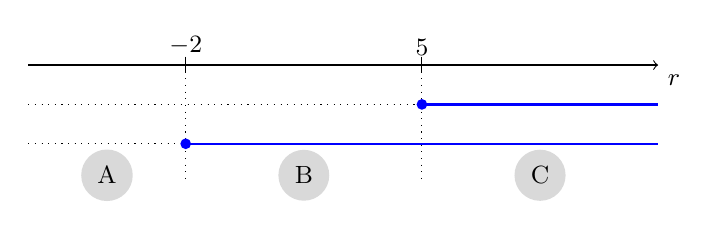
\begin{tikzpicture}[font=\small,x=10mm, y=10mm]

\draw[->] (0,0) -- (8,0) node [below right] () {$r$};

\foreach \x in {2,5}{
\draw(\x,3pt)--(\x,-3pt);
\begin{scope}[dotted]
\draw (\x,0) -- (\x,-1.5);
\draw (0,-.5) -- (5,-.5);
\draw (0,-1) -- (2,-1);
\end{scope}}

\node[above]  at (5,0) {$5$};
\node[above]  at (2,0) {$-2$};
\node [circle,fill=gray!30](A) at (1,-1.4) {A};
\node [circle,fill=gray!30](B) at (3.5,-1.4) {B};
\node [circle,fill=gray!30](C) at (6.5,-1.4) {C};

\begin{scope}[blue,thick]
\draw (5,-.5) -- (8,-.5);
\draw (2,-1) -- (8,-1);


\draw[fill=blue] (5,-.5)circle (1.5pt);
\draw[fill=blue] (2,-1)circle (1.5pt);

\end{scope}

\end{tikzpicture}

% \end{center}
% 
% \begin{enumerate}[label={(\Alph*)}]
%  \item $x<-2$: in questo intervallo entrambi gli argomenti sono negativi, 
% pertanto 
% \[f(x)=\valass{x-5}+\valass{x+2}=-x+5-x-2=-2x+3.\]
% Se $x=-2$ si ha $f(-2)=\valass{-2-5}+0=7$
%  \item $-2<x<5$ il primo argomento è negativo e il secondo è positivo, pertanto 
% \[f(x)=\valass{x-5}+\valass{x+2}=-x+5+x+2=7.\]
% Se $x=5$ si ha $f(5)=0+\valass{5+2}=7$
%  \item $x>5$ entrambi gli argomenti positivi, pertanto 
% \[f(x)=\valass{x-5}+\valass{x+2}=x-5+x+2=2x-3.\]
% \end{enumerate}
% Possiamo allora sintetizzare in questo modo
% \[
% \valass{x-5}+\valass{x+2}=\left\{\begin{array}{l}
% -2x+3 \text{, se }x<-2\\
% 7 \text{, se }-2\le x<5\\
% 2x-3 \text{, se }x\ge 5\end{array}.\right.
% \]
% \end{esempio}
\end{exrig}
% \ovalbox{\risolvii \ref{ese:1.7}, \ref{ese:1.8}, \ref{ese:1.9}, 
% \ref{ese:1.10}, \ref{ese:1.11}}
